\hypertarget{stm32f4xx__hal__dma_8c}{}\section{Dokumentacja pliku S\+T\+M/\+W\+D\+S\+\_\+\+Kosc\+\_\+\+Linux/\+Drivers/\+S\+T\+M32\+F4xx\+\_\+\+H\+A\+L\+\_\+\+Driver/\+Src/stm32f4xx\+\_\+hal\+\_\+dma.c}
\label{stm32f4xx__hal__dma_8c}\index{S\+T\+M/\+W\+D\+S\+\_\+\+Kosc\+\_\+\+Linux/\+Drivers/\+S\+T\+M32\+F4xx\+\_\+\+H\+A\+L\+\_\+\+Driver/\+Src/stm32f4xx\+\_\+hal\+\_\+dma.\+c@{S\+T\+M/\+W\+D\+S\+\_\+\+Kosc\+\_\+\+Linux/\+Drivers/\+S\+T\+M32\+F4xx\+\_\+\+H\+A\+L\+\_\+\+Driver/\+Src/stm32f4xx\+\_\+hal\+\_\+dma.\+c}}


D\+MA H\+AL module driver.  


{\ttfamily \#include \char`\"{}stm32f4xx\+\_\+hal.\+h\char`\"{}}\newline
Wykres zależności załączania dla stm32f4xx\+\_\+hal\+\_\+dma.\+c\+:\nopagebreak
\begin{figure}[H]
\begin{center}
\leavevmode
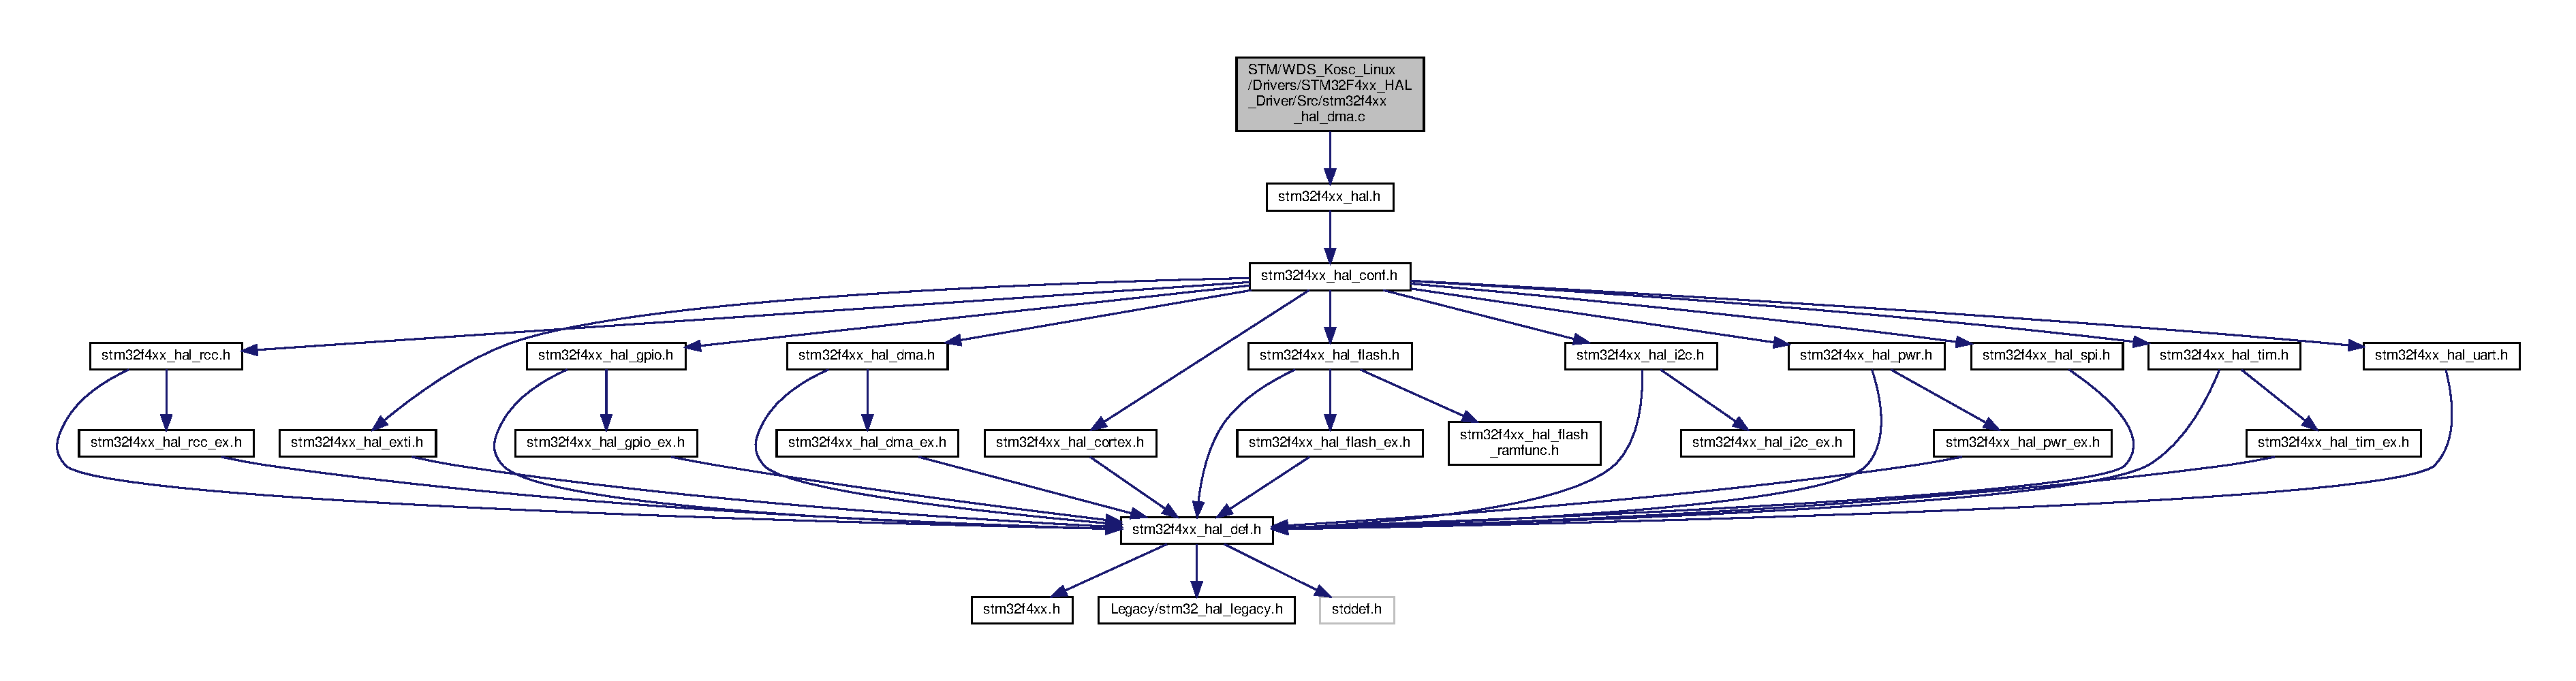
\includegraphics[width=350pt]{stm32f4xx__hal__dma_8c__incl}
\end{center}
\end{figure}


\subsection{Opis szczegółowy}
D\+MA H\+AL module driver. 

\begin{DoxyAuthor}{Autor}
M\+CD Application Team This file provides firmware functions to manage the following functionalities of the Direct Memory Access (D\+MA) peripheral\+:
\begin{DoxyItemize}
\item Initialization and de-\/initialization functions
\item IO operation functions
\item Peripheral State and errors functions \begin{DoxyVerb}==============================================================================
                      ##### How to use this driver #####
==============================================================================
[..]
 (#) Enable and configure the peripheral to be connected to the DMA Stream
     (except for internal SRAM/FLASH memories: no initialization is 
     necessary) please refer to Reference manual for connection between peripherals
     and DMA requests.

 (#) For a given Stream, program the required configuration through the following parameters:
     Transfer Direction, Source and Destination data formats, 
     Circular, Normal or peripheral flow control mode, Stream Priority level, 
     Source and Destination Increment mode, FIFO mode and its Threshold (if needed), 
     Burst mode for Source and/or Destination (if needed) using HAL_DMA_Init() function.

 -@-   Prior to HAL_DMA_Init() the clock must be enabled for DMA through the following macros:
       __HAL_RCC_DMA1_CLK_ENABLE() or __HAL_RCC_DMA2_CLK_ENABLE().

   *** Polling mode IO operation ***
   =================================
  [..]
        (+) Use HAL_DMA_Start() to start DMA transfer after the configuration of Source 
            address and destination address and the Length of data to be transferred.
        (+) Use HAL_DMA_PollForTransfer() to poll for the end of current transfer, in this  
            case a fixed Timeout can be configured by User depending from his application.
        (+) Use HAL_DMA_Abort() function to abort the current transfer.

   *** Interrupt mode IO operation ***
   ===================================
  [..]
        (+) Configure the DMA interrupt priority using HAL_NVIC_SetPriority()
        (+) Enable the DMA IRQ handler using HAL_NVIC_EnableIRQ() 
        (+) Use HAL_DMA_Start_IT() to start DMA transfer after the configuration of  
            Source address and destination address and the Length of data to be transferred. In this 
            case the DMA interrupt is configured 
        (+) Use HAL_DMA_IRQHandler() called under DMA_IRQHandler() Interrupt subroutine
        (+) At the end of data transfer HAL_DMA_IRQHandler() function is executed and user can 
            add his own function by customization of function pointer XferCpltCallback and 
            XferErrorCallback (i.e a member of DMA handle structure).
  [..]
   (#) Use HAL_DMA_GetState() function to return the DMA state and HAL_DMA_GetError() in case of error 
       detection.

   (#) Use HAL_DMA_Abort_IT() function to abort the current transfer

   -@-   In Memory-to-Memory transfer mode, Circular mode is not allowed.

   -@-   The FIFO is used mainly to reduce bus usage and to allow data packing/unpacking: it is
         possible to set different Data Sizes for the Peripheral and the Memory (ie. you can set
         Half-Word data size for the peripheral to access its data register and set Word data size
         for the Memory to gain in access time. Each two half words will be packed and written in
         a single access to a Word in the Memory).

   -@-   When FIFO is disabled, it is not allowed to configure different Data Sizes for Source
         and Destination. In this case the Peripheral Data Size will be applied to both Source
         and Destination.

   *** DMA HAL driver macros list ***
   =============================================
   [..]
     Below the list of most used macros in DMA HAL driver.
     
    (+) __HAL_DMA_ENABLE: Enable the specified DMA Stream.
    (+) __HAL_DMA_DISABLE: Disable the specified DMA Stream.
    (+) __HAL_DMA_GET_IT_SOURCE: Check whether the specified DMA Stream interrupt has occurred or not. 

   [..]
    (@) You can refer to the DMA HAL driver header file for more useful macros\end{DoxyVerb}

\end{DoxyItemize}
\end{DoxyAuthor}
\begin{DoxyAttention}{Uwaga}

\end{DoxyAttention}
\subsubsection*{\begin{center}\copyright{} Copyright (c) 2017 S\+T\+Microelectronics. All rights reserved.\end{center} }

This software component is licensed by ST under B\+SD 3-\/\+Clause license, the \char`\"{}\+License\char`\"{}; You may not use this file except in compliance with the License. You may obtain a copy of the License at\+: opensource.\+org/licenses/\+B\+S\+D-\/3-\/\+Clause 